%
%
%
%
%
%
%
%
%
%
%
%
%
%
%
%
%
\begin{document}
\maketitle
\begin{abstract}
\end{abstract}

\section{Introduction} 

% (fold)
\label{sec:introduction}

Suppose that you wanted to make the following argument: 
\begin{hypo}
	\label{h1} A particular property of a brain causes a particular mental property. 
\end{hypo}

The ``brain property'' could be nearly anything: the genetic expression profile of a subset of neurons in a particular developmental stage, or microtubules becoming entangled, or columnar organization, or the bumps in our skulls, etc. Similarly, the ``mental property'' could be almost anything: intelligence, capacity for love, knowing the square-root of pi, etc. How might you go about \emph{proving} Hypothesis \ref{h1} (H\ref{h1})?

Here's how we would do it. First, we would change H1 to be \emph{testable}, and change our desiderata from \emph{proving} its accuracy to \emph{collecting evidence} to support its claim. More specifically, we would make the following argument:
\begin{hypo}
	\label{h2} A change in particular property of a brain can predict a corresponding change in a particular mental property\footnote{Note the relationship between this and \emph{statistical-supervenience} \cite{VogelsteinPriebe10}}. 
\end{hypo}

Now, to collect evidence in support of H\ref{h2}, we need the following:
\begin{enumerate}
	\item A way to describe any brain, $b$. Our description should live in the space of all possible descriptions of brains (or, at least those under consideration), $\mB$. 
	\item A way to describe a mental property, $m$, which lives in the space of mental properties, $\mM$. For instance, if the mental property under investigation is IQ, then $\mM$ may be all possible scores on a particular IQ test. 
	\item A mapping from brain space to mental space, which enables us to relate $m$ and $b$. Call this mapping, $g$, so $g: \mB \mapsto \mM$. 
\end{enumerate}

If we choose to take a statistical perspective, then both brains and minds are random variables. More specifically, let $B$ be a random variable corresponding to a brain, so that any particular brain, $b$, is a sample from the space of brains, $\mB$. The probability of $B$ taking any value $b \in \mB$ is given by the \emph{marginal} distribution $F_B[b = B)$%, where $\int_{b\in\mB} F_B(b=B)db=1$, and $P_B(b=B)\geq 0 \, \forall b \in \mB$
. Similarly, let $M$ be a random variable corresponding to the mental property under investigation, so $m$ is a sample from the space of mental properties, $\mM$. The probability of $M$ taking any value $m \in \mM$ is given by the \emph{prior} distribution $F_M(m = M)$. The mapping, $g$, tells us the relationship between any $m$ and any $b$. Or, more formally, the mapping tells us about the \emph{posterior} distribution of minds given brains, $F_{M|B}(m=M | b=B)$. 

If we knew the \emph{joint} distribution of minds and brains, $F_{BM}(b=B,m=M)$, and the marginal distribution of brains, $F_B$, then finding the mapping from brains to minds would be trivial: we would simply use Bayes rule to obtain the posterior, $F_{M|B} = F_{BM}/F_B$. However, in practice these distributions are typically unknown. Therefore, we must \emph{estimate} $g$ from a corpus \emph{data}. Assume we have collected $n$ brain/mental pairs. Then, define the corpus of data as the collection of all such pairs: $\mD_n=\{(b^1,m^1), \ldots, (b^n,m^n)\}$. The estimated mapping, $g_n$, then takes a new brain and the old \emph{training data}, and makes predictions about the mental property $m$. Formally, $g_n: \mB \times (\mB, \mM)^n \mapsto \mM$, so $g_n(b; \mD_n)=\hm$.

This work contributes a perspective on a possible space of brains, $\mB$, and several principled ways of choosing $g_n$. In so doing, we also describe a set of desiderata for both $\mB$ and $g_n$ to satisfy. We make no claim that our definitions or desiderata are novel or unique. Rather, the novel contribution (if any), is the overarching statistical perspective that unifies previously (potentially) disparate ideas into a single coherent framework.

% section introduction (end)
\section{A possible description of brains with certain desirable properties} 

% (fold)
\label{sec:B}

Many possible spaces for the descriptions of brains exist. For instance, phrenologists thought that the ``sulci and gyri'' of the \emph{skull} were sufficient to explain various mental properties, including intelligence. The space of brains they considered then, were all possible skull shapes. Clearly, such a space is not sufficient to compare the evidence support phrenological theory with an alternate theory, such as it is the sulci and gyri of the \emph{brain} that determine those mental properties. So, can we enumerate a set of desiderata which we would use to select our brain-space? Here is a possible set:
\begin{enumerate}
	\item $\mB$ should be sufficiently large to be able account for whatever properties of the brain are casually related to the properties of cognition under investigation. 
	\item $\mB$ should be sufficiently large to be able span multiple \emph{levels of explanation}. That is, we might want to be able to compare a hypothesis about the role of genetic expression profiles with another hypothesis about default mode networks. 
	\item $\mB$ should be only as large as necessary, and no larger. In particular, if we do not believe that total brain volume can \emph{cause} a particular mental property, that it need not be included. 
	\item The properties of any particular brain, $b\in \mB$, should be either measurable or estimatable, such that experimental observation may be used to obtain them.	% \item Parameter estimates should be consistent \cite{?} %, that is, $\hbth_n \conv \theta$ as $n \conv \infty$.
	\item $\mB$ should admit algorithms that (are guaranteed to be able to) capture the relationship of interest. 
%	\item $\mB$ should also admit \emph{causal} studies, which entail modifying a particular $b \in \mB$, to modify the corresponding mental property, $m \in \mM$. 
\end{enumerate}

Note that the above desiderata are neither complete nor unique; rather, they provide (hopefully) a reasonable set of criteria for evaluating any proposed $\mB$. 
% \section{Paradigms of research} (fold)
% \subsection{Current Paradigm}
% 
% The dominant paradigm of quantitative neuroscience in the 20$^{th}$ century has been the ``signal processing'' framework \cite{?}.  Essentially, the brain is a box, that filters some stimulus, to produce some response (see Figure 1). This framework leads to the following goal:
% 
% \begin{goal}
% 	Learn the filter that the brain performs on stimuli to result in the actualized responses.
% \end{goal}
% 
% \begin{figure}[h!)
% \centering 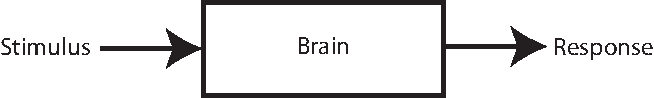
\includegraphics{stim_brain_resp}
% \caption{The signal-processing paradigm of quantitative neuroscience.  The brain is a box that essentially \emph{filters} the stimulus, outputting some response, which is often take to be multivariate time series (such as populations of spike trains or fMRI activity).} \label{fig:SBR}
% \end{figure}
% 
% 
% This paradigm has been appropriate, given the kind of data available to people investigating the brain.  More specifically, the kind of data that has been most available has been time-series of signals related to neural activity \cite{?}.  Given that electrical engineers were largely the individuals obtaining and analyzing the data, it was natural to take a signal-processing approach.  Often, the dynamic time-series data were used to estimate static parameters.  In the previous decades, these communities have been more and more sophisticated models and algorithms to estimate these parameters \cite{?}.  Recently, issues such as parameter identifiability, consistency, bias, and model selection have been gaining traction as important desiderata for our models \cite{?}.  
% 
% \subsection{Alternate Paradigm}
% 
% Here, we define a different goal, which suggests a complementary research paradigm to the current dogma: %which we believe has not been satisfied by any previously proposed research paradigm.  Further, we elaborate on a novel paradigm that we believe is sufficient to satisfy this goal.
% 
% \begin{goal}
% 	Construct a family of brain-models, $\mB$, that is sufficient to provide \emph{causal} explanations relating properties of minds with properties of brains.
% \end{goal}
% 
% Note how the above goal is distinct in certain respects from the ``filtering'' goal.  First, neither stimulus nor response is explicitly incorporated into this goal.  While stimuli and response may be used as tools to obtain the parameters of $\mB$, that is their only merit in this paradigm.  Second, minds are explicitly incorporated into this goal.  While spike trains or fMRI signal may indicate mental processes, they are likely not what is meant by ``mind''; rather, they may be used as tools to infer mental states.  Third, the inclusion of a class of models $\mB$  suggests a statistical \emph{static} framework, rather than a dynamics perspective.  In addition to the above stated goal, we would like the family of models $\mB$ to satisfy a number of desiderata:
% 
% \begin{enumerate}
% 	\item $\mB$ %$=\{\mathbb{P}_{\theta}; \theta \in \Theta\}$ 
% 	should be sufficiently general to account for whatever properties of the brain are casually related to the properties of cognition under investigation.
% 	\item The properties of any particular brain, $b\in \mB$, should be either measurable or estimatable, such that experimental observation may be used to obtain them.
% 	% \item Parameter estimates should be consistent \cite{?} %, that is, $\hbth_n \conv \theta$ as $n \conv \infty$.
% 	\item $\mB$ should admit algorithms that (are guaranteed to be able to) capture the relationship of interest.
% 	\item $\mB$ should also admit \emph{causal} studies, which entail modifying a particular $b \in \mB$, to modify the corresponding mental property, $m \in \mM$.
% \end{enumerate}
% 
% \section{NeuroCognitive Graph Theory}
% 
% \subsection{Brain-graphs}
% 
% Here, (end)
With this in mind, we propose the notion of a \emph{brain-graph}. Specifically, we say that the brain may be well characterized as a labeled, attributed multigraph (which is a generalized notion of a or network). Formally, we define a brain-graph, $b\in \mB$ as a 4-tuple, $\mB=(\mV,\mE,\mX_V, \mX_E)$, defined by the following:
\begin{itemize}
	\item The set of vertices (nodes), $V=\{V_i\}_{i\in[n_v]}$. If we assume, for instance, that neurons are the fundamental (atomic) unit of computation, then each vertex could correspond to a neuron. Regardless of what vertices represent, formally, we let $V_i \in \mV_i = \{0,1\}$ for $i \in [n_v]=\{1,2,\ldots,n_v\}$, $n_v \leq \infty$, and $\mV = \mV_i^{n_v}$.	%$=\{V_i\}$, where $V_i \in \mV \subseteq \mathbb{Z}$ . 	
	\item The set of edges, $E=\{E_{ij}\}_{i,j \in [n_v]}$. Again, if we assume that neurons are the fundamental unit of computation, then each edge could correspond to a synapse. To simplify matters we may only consider the presence or absence of a synapse, in which case $E_{ij} \in \{0,1\}$. Or, we may consider the effective strength of a synapse, in which case $E_{ij} \in \mathbb{Z}$, where $\mathbb{Z}$ is the set of integers, $\{0,1,2,\ldots\}$. Further, we could allow for the possibility of multiple ``kinds'' of synapses between any pair of neurons, such as chemical and electrical. In such a case, we have $E_{ijk} \in \mE_{ijk} \subseteq [n_v]^2 \times [n_k]$, where $n_k\leq \infty$ is the maximum number of categorically different edges. In any case, we can define the space of edges as $\mE=\mE_{ijk}^{n_v^2 \times n_k}$. 	%, where $E_{ij} \in \mE_{ij} \subseteq \mathbb{Z}$ for $(i,j) \in [n_v] \times [n_v]$, so $\mE = \mE_{ij}^{n_v^2}$.  If edges are undirected, then $E_{ij}=E_{ji}$.  If edges are binary, then $\mE=\{0,1\}$.  If we have multi-edges corresponding to categorically different edges (such as electrical and chemical synapses), each edge may also be indexed by $k \in \mathbb{Z}$. If multi-edges correspond to integer weighted edges, then $\mE$ is the set of allowable integers (which may be countably infinite).
	\item If vertices have features (or labels/attributes), then let $X_i$ correspond to the feature vector for vertex $i$ %, and define $X=\{X_i\}_{i \in [n_v]}$. 
(features may correspond to \emph{anything} about the vertex). Again, assuming vertices represent neurons, features may indicate neurotransmitter released, morphological properties, receptive fields, etc. Formally, $X_i \in \mX_1 \subseteq \Real^{d_V}$ for $i \in [n_v]$, and $d_V$ is the dimensionality of the feature vectors, so $\mX_V = \mX_1^{n_v}$. It may be the case that certain features are measurable/observable, and others are hidden. If so, let $X_i = X^o_i \cup X^h_o$, and $X^o_i \cap X^h_i = \emptyset$. 
	\item If edges also have features, then let $X_{ij}$ correspond to the feature vector for edge $(i,j)$.  If edges are synapses, then edge features might include things like probability of release, post-synaptic potential shape, etc. Let $X_{ij} \in \mX_2 \subseteq \Real^{d_E}$ for $(i,j) \in [n_v] \times [n_v]$, and $d_E$ is the dimensionality of the edge features, so $\mX_E=\mX_2^{n_v^2}$. In the scenario where categorically different edges exist, let an additional index $k$ indicates edge features for each category $k$, so $\mX_E=\mX_2^{n_v^2 \times n_k}$.
\end{itemize}

Given such a brain-space $\mB$, a natural question is: does this notion of brain-graphs satisfy the above desiderata? Let's see:

\begin{enumerate}
	\item The space of all possible brain-graphs does appear to be quite large, potentially incorporating many small and large details of brains.
	\item Because each vertex $V_i$ could correspond to a neuron, a column, a neuroanatomical region, etc., indeed, brain-graphs can span multiple levels of explanation.  Even for a given brain, it is possible to let some $V_i$'s represent neurons, and other $V_i$'s represent neuroanatomical regions, even if this is a redundant characterization of the brain, in that the neurons are \emph{within} the neuroanatomical region.
	\item While the brain-graph space is large, it is not ``all-encompassing.''  For instance, the space of all possible functions is not within brain-graph space. Thus, the brain-graph space seems to exclude at least some possibilities.
	\item For a space to admit algorithms guaranteed to capture the relationship of interest, one must prove limiting results.  For instance, Stone proved in 1977 \cite{Stone77} that the $k_n$ nearest neighbor algorithm is guaranteed to converge to the Bayes optimal solution.  In 2010, Vogelstein et al. \cite{VogelsteinPriebe10} proved a similar result holds for brain-graphs.
%	\item Brain-graphs clearly admit causal studies, as one could modify the number of nodes, or the value of edges or features, and (potentially) observe a corresponding change in a mental property.  
\end{enumerate}

Note one significant omission in the above is any \emph{dynamic} notion, that is, the above brain-graph description is entirely \emph{static}\cite{?}.  This fact is easily remedied by introducing an index $t$ into the space, i.e., $\mB_t$, so the entire space can be time-varying.  This more general notion of \emph{dynamic} brain-graphs will be addressed in future work.

Thus, it seems that brain-graphs indeed satisfy the above criteria.  This is not to say that brain-graphs are the only space one could define to satisfy these criteria, merely that brain-graphs are sufficient. So, given such a space of brains, the next question is: ``how can one choose a mapping between brains and minds?''


%Assume, for the moment, that we take the fundamental computational unit of the brain to be a point neuron. Then, each vertex is a neuron, and each edge is a synapse. Categorically different edges may correspond to chemical and electrical synapses. Vertex attributes could include neurotransmitter released, proteins expressed, morphological properties, receptive fields, etc. Edge attributes could include probability of release, post-synaptic potential shape, etc. This level of description, however, is not necessary. For instance, $\mV$ might instead correspond to neuroanatomical regions, which admit very different notions for edges and attributes. This multi-scale aspect of $\mB$ is an important advantage over other frameworks. 

% section a_possible_description_of_brains_with_certain_desirable_properties (end)

\section{Possible approaches to choosing mappings with desirable properties}  % (fold)
\label{sec:map}

Given $\mB$, what can we do with it? As stated above, our goal is to relate these models to properties of cognition. More specifically, let $\mM$ characterize the space of the mental (cognitive) property, and $g \in \mG$ be some mapping to learn. Then $g: \mB \conv \{0,1,\ldots,C\}$ is a $C-$way classifier. 
% \begin{itemize}
% 	\item If $\mM=\{0,1\}$, then $g$ may be a two-way classifier: $g: \mB \conv \{0,1\}$. 
% 	\item If $\mM=\{0,1,\ldots, n_m\}$, then $g$ may be an $n_m-$way classifier: $g: \mB \conv \{0,1,\ldots,n_m\}$. 
% 	\item If $\mM=\Real^a$, then $g$ is a (multivariate-) regressor: $g: \mB \conv \Real^a$. 
% \end{itemize}
As discussed above, solving these problems---which means finding $g$---will depend on the joint distribution of brains and minds, $F=F_{BM}$. Because $F_{MB}$ is typically unknown, $g$ must be estimated, using some training data, $\mD_n$, to obtain $g_n(b; \mD_n)$. The particular $g_n$ should be the one that minimizes some loss function, $L_F(g_n)$, over the space of all possible $g_n$'s, $\mG$. For instance, when $|\mM|=2$, $\mG$ is all possible two-way classifiers, and a potentially reasonable loss function is $L_F(g_n)=\mathbb{E}[P_F(g_n(B;\mD_n) \neq M | \mD_n)]$. %Importantly, in addition to finding a $g_n$ that minimizes some loss-function, $g_n$ should admit a way to \emph{morph} any brain's mental property $m$, by modifying $b$. This will be discussed at greater length in the sequel. 

% \subsection{Finding a good $g_n$} % (fold)
% \label{sub:finding_a_good_g_n_}

Thus, given a mental property, a decision about how to represent it, $\mM$, and a loss function, $L$, our task is to find a good algorithm, $g_n$. Two complementary strategies are possible: model-free and model-based. Model-free algorithms have the advantage that no model need be specified. %Thus, in theory, model-free algorithms have the advantage of having little or no bias. Unfortunately, this freedom comes with the cost of relatively high variance. 
Unfortunately, these models often provide very little intuition (if any) about the underlying causes of the relationship of interest, and therefore lack \emph{interpretability}.  On the other hand, model-based algorithms can provide rather simple interpretations.  However, model-based algorithms require defining a space of models sufficient to capture the relevant aspects of $\mB$.  Classes of models sufficiently large to span $\mB$ often have large variance, and suffer from over-fitting issues.  %On the other hand, model-based algorithms can significantly reduce variance, but (almost) necessarily increase bias. Importantly, 
Note that many standard algorithms including linear, quadratic, and support vector based classifiers/regressors \emph{implicitly} define a model, and are therefore not strictly ``model-free''.

\subsection{Model-free algorithms} % (fold)
\label{sub:model_free_algorithms}

Model-free algorithms often operate on interpoint distance space, as opposed to the explicit data space \cite{MaaBartoszynski96}. More formally, given any two brain-graphs, $b^1$ and $b^2$, first define an interpoint (pseudo-) distance metric: $\rho: \mB \times \mB \mapsto [0,\infty)$. This reduces the problem from operating in $\mB$ to operating in $\Real_+$. Because the data collected is often corrupted by noise, it is typical to also introduce a smoothing function: $s: \mB \mapsto \mB$. For the brain-graph scenario, this may correspond to inferring unobserved edges. Thus, the smoothing-derived (pseudo-) distance metric, $\rho'$ is defined as: $\rho' = \rho(s(b^1),s(b^2))$. 

Perhaps the prototypical model-free algorithm is the $k_n$ nearest neighbor (kNN) algorithm. Vogelstein et al. (2010) showed that a kNN classifier is a universally consistent classifier (meaning, achieves the Bayes optimal performance), for any $F_{BM}$, under a Frobenius norm distance metric. In other words, they let defined $\rho(\cdot)=\norm{\cdot}_F$, and $s$ was simply the identity (that is, no smoothing). Simulations showed that for only a few hundred simulated sample data points, this kNN achieved misclassification error rate below 10\%. In practice, it is often the case that other model-free algorithms outperform (in accuracy) any particular kNN, including class cover catch digraphs, decision trees, and various ensemble approaches such as random forests \cite{Breiman01}. Unfortunately, scant theoretical works is available to provide proofs of universal consistency for these alternate model-free algorithms \cite{?}.

%While this is a desirable property, our belief is that other $g_n$'s may outperform the kNN classifier on finite data sets.  More specifically, while kNN induces no bias whatever into $g_n$, the variance is large.  Thus, by incorporating neuroscientific knowledge about these brain-graphs into $g_n$, it may be possible to only marginally increase the bias, but drastically reduce the variance, yielding improved performance.  

% subsection model_free_algorithms (end)

\subsection{Model-based algorithm}  % (fold)
\label{sub:model_based_algorithm}

The other possible strategy is to propose a class of models, $\mP=\{P_{\theta} : \theta \in \Theta \subseteq \Real^d\}$, that describe the data (note that the choice of how to determine the dimensionality $d$ of the model specifies whether the model is parametric, semiparametric, or nonparametric).  Like the class of brain-graphs, $\mB$, the class of models, $\mP$, should satisfy several desiderata:

\begin{enumerate}
	\item Lower dimensional $\Theta$ are preferred over higher dimensional $\Theta$, \emph{ceteris parabus}.
	\item As the number of data points approaches infinity, so should the dimensionality of the model, that is:  $n \conv \infty \implies d\conv \infty$.
	\item $\theta$ should be at least \emph{generically identifiable} \cite{AllmanRhodes10}.
	\item Estimators for $\theta$ should be consistent \cite{DGL96}.
\end{enumerate}


% Ideally, the class of models is sufficiently large to include models very close to the ``truth''.  The goal is then to find a Minimally Sufficient Model (MSM; by analogy with minimally sufficient statistics) within the class, that sufficiently explains the data.  The ability to obtain a \emph{consistent} estimator of $\theta$ is , with the ``smallest'' $\Theta$ (a potentially useful measure of size is the set cardinality). %goes to infinity as $n$ goes to infinity.   
% The advantage of using a semiparametric model is the amount of bias introduced by the model is a function of the amount of data available, that is, given infinite data, they can be bias free. The goal then is to find a Minimally Sufficient Model (MSM; by analogy with minimally sufficient statistics), which is the brain-graph with the least parameters that explains the mental property under investigation sufficiently.  %$g_n$ then operates directly on $\hbth$, the data dependent estimate of the model parameters, $\theta$. 
% Given this estimate, classification/regression with $g_n$ is then performed on the estimate of $\theta$, which lives in some $\Theta$ space smaller than $\mB$, thereby reducing the variance, without increasing bias too much (hopefully).
Model-based approaches therefore have a multi-step process: (i) define $\mP$, (ii) fit the model by finding $\hbth \in \Theta$ that minimizes some loss function, and (iii) find/compute $g_n(\hbth)$ that minimizes some other loss function\footnote{Is it interesting to note that neither paradigm actually operates directly on the data? The model-free approach operates on $\rho$, and the model-based approach operates on $\hbth$.}.  
%The model-based approach also (potentially) offers the advantage of \emph{interpretability}, if the parameters, $\theta$, correspond to interpretable features of the brain. 
% Let $b^i$ correspond to brain-graph $i$. The model-based approach then typically assumes that each $b^i$ is sampled identically and independently from some parametric distribution, $b^i \overset{iid}{\sim} P(b^i | \theta) \, \forall i \in [n]$. Because $\theta$ is typically unknown, an estimate, $\hbth$, must be found. Given such an estimate, $g_n$ operates directly on the estimated parameters, as opposed to the brain-graphs 
Below, we describe several possible model classes, $\mP$, with increasing complexity.  For each, a heuristic for how to fit the model is provided.  Given that these are model-based approaches, each class of models admits a posterior distribution, $P(m | \hbth)$.  Thus, $g_n$ will always provide the maximum a posteriori estimate of $m$, or some close approximation to it. %In the below examples, we deal exclusively with the classification setting, leaving regression to future work.  %The decision of to find $g_n$ given $\hbth$ is mostly a pragmatic issue: which ever one works best given $\hbth$ is the one to use.  Thus, the third step is given relatively short shrift here.  Throughout, we assume that the number of vertices, $n_v$ is fixed and given for all brain-graphs under consideration (for simplicity).  This assumption is easily relaxed.

\subsubsection{Edge independent models} % (fold)
\label{ssub:edge_indep}

The first class of models we consider greatly simplifies the brain-space.  Specifically, we make the following simplifying assumptions:

\begin{enumerate}
	\item the number of vertices is known and fixed for all brain-graphs
	\item each edge is independent and distributed according to the same parametric family of distributions
	\item vertex and edge features do not contain any useful information with regard to $M$
\end{enumerate}

Given these three assumptions, each brain is completely characterized by its adjacency matrix.  Let $e^l$ indicate the adjacency matrix for brain $l$, that is $e^l=\{e_{ij} | e_{ij} \in e^l\} \overset{iid}{\sim} P_E(\cdot | \theta)$.
% 
% Let $E^l$ indicate the adjacency matrix for brain $i$. We can formally write the model, therefore, as:
% \begin{align}
% 	P(b^l|\theta) = P(E^l | \theta) = \prod_{(i,j)\in E^l} P(E^l_{ij} | \theta)
% \end{align}
% 
If each edge identically distributed, then $\theta$ is a scalar. Otherwise, $\theta$ is a vector, with up to $n_v^2$ parameters.  Because $\mE$ is the space of multi-edges, each each $e^l_{ij}$ potentially takes any integer value.  Thus, any discrete probability mass function is possible.  To satisfy the above desiderata, however, exponential family distributions are preferred, as they admit identifiable and consistent estimators.  Furthermore, if a Bayesian perspective is taken, exponential family distributions admit conjugate priors, meaning that maximum a posteriori estimates may be obtained, assuming an appropriate prior is available.  For instance, a reasonable model may be that edges are sampled from a Poisson distribution, and the parameters of the Poisson come from a Gamma distribution.  The prior can incorporate knowledge, for instance, that brain-graphs tend to be rather sparse \cite{?}.  

For example, assume that we have classes $0,1,\ldots, C$, and edges can take any integer value.  Then,  $\theta=\{\lam_0,\lam_1, \ldots, \lam_C\}$, corresponding to the expected weight of any edge in class $c$.  Further assume  that the hyperparameters $\{\alpha,\beta\}$ are known, and the same across classes.  To estimate $\lam_c$, we have:

\begin{align}
	\hlam_c &= \argmax_{\lam_c \geq 0}  \prod_{l | m^l = c} P(\lam_c | b^l) = \argmax_{\lam_c \geq 0}  \bigg(\prod_{l | m^l=c} P(b^l | \lam_c)\bigg) P(\lam_c) = \argmax_{\lam_c \geq 0}     \prod_{\substack{l | m^l = c \\ (i,j) \in E^l}} P_E(e^l_{ij} | \lam_c) P(\lam_c)\nonumber \\
	&= \argmax_{\lam_c \geq 0} \prod_{\substack{l | m^l = c \\ (i,j) \in E^l}}  \text{Poisson}(e^l_{ij}; \lambda_c) \text{Gamma}(\lam_c; \alpha, \beta) \nonumber \\ 
	&= \argmax_{\lam_c \geq 0} \prod_{\substack{l | m^l = c \\ (i,j) \in e^l}} \text{Gamma}(\lam_c; \alpha + \sum_{\substack{l | m^l = c \\ (i,j)\in e^l}} e^l_{ij}, \beta + \sum_{l \in [n]}|e^l| ).
	%\frac{ \lam^{E^l_{ij}}\exp\{-\lam\} }{E^l_{ij}!} \lam^{\alpha-1} \frac{\exp\{-\lam \beta \}}{\Gam(\alpha)/\beta} = \argmax_{\lam \geq 0} \prod_{\substack{l \in [n] \\ (i,j) \in E^l}} 
\end{align}
Once we obtain $\hth=\{\hlam_0,\hlam_1,\ldots, \hlam_C\}$, given a new brain, $b$, classifying $b$ is trivial:
\begin{align}
	\hm &= g_n(b; \mD_n, \hth) = \argmax_{c \in [C]} \{P_E(b | \hlam_c)\} %\nonumber \\& 
	= \argmax_{c\in[C]} \prod_{(i,j)\in e}\text{Poisson}(e_{ij}; \hlam_c).
\end{align}
This strategy, of course, can be easily generalized in a number of ways.  First, $\lam$ could be a function of edge identity, instead of the same across all edges.  Second, the hyperparameters could be different across classes.  Third,  the hyperparameters can be estimated using, for instance, cross-validation.  Note that for numerical reasons, we typically use log posteriors, requiring a summation instead of multiplication of many potentially small numbers.


Unfortunately, while tractable and simple, this model does not satisfy all of our above desiderata with respect to $\mP$.  In particular, this is a \emph{parametric} model, meaning that the number of parameters is necessarily \emph{finite} ($\leq n_v^2$).  Thus, while this model can act as a \naive base model, more sophisticated models are desirable.  


% subsubsection edge_independent_models (end)

\subsubsection{Edge conditionally independent model} % (fold)
\label{ssub:edge_cond}


In Section \ref{ssub:edge_indep}, we defined a very simple model, completely neglecting all features, and assuming the each edge is independent.  For many data sets, making either of these assumptions (and all the more so for both of these assumptions) will not yield satisfactory descriptions of the data \cite{?}.  Here, we relax the last two assumptions.  Rather, the probability of each edge is only a function of the feature vectors for the two vertices that define the edge, and the feature vector of the edge.  In this model, edges are not independent, but they are \emph{conditionally independent} given the features.   Formally, let $x$

we say:
\begin{align}
	P(b^l | \theta) &= P(e^l, x^l | \theta) = P_E(e^l | x^l) P_X(x^l | \theta) 
	% \\ &=\prod_{(i,j) \in e^l} P_{E}[e_{ij}^l | x^l) P_X(x^l | \theta)\\
	% &= \prod_{(i,j) \in e^l} P_{E}[e_{ij}^l | x^l) P_{X_E} [x^l_{ij} | \theta ) \prod_{i\in[n_v]} P_{X_V}(x^l_i | \theta) 
\end{align}
% Importantly, the feature distribution, $P_X(x^l | \theta)$ factorizes into vertex and edge features, and both further factorize:
% \begin{align}
% 	P_X(x^l | \theta) = P_{X_V}(x^l_V | \theta) P_{X_E}(x^l_E | \theta) = \prod_{i\in[n_v]} P_{X_V}(x^l_i | \theta) \prod_{(i,j)\in e^l}P_{X_E}(x^l_{ij} | \theta) 
% \end{align}
Assuming that all edges and features are observed, and we have classes $\{0,1,\ldots,C\}$, yielding conditional parameters, $\{\theta_0$, $\theta_1$, $\ldots$, $\theta_C\}$, then we can estimate the parameters for this model, for any particular class $c$:
\begin{align}
	\widehat{\theta}_c 	&= \argmax_{\theta_c \in \Theta} \prod_{l | m^l=c} P(\theta_c | e^l, x^l) %\nonumber \\ &
			= \argmax_{\theta_c \in \Theta} \prod_{l | m^l=c} P(e^l, x^l | \theta_c) P_{\theta}(\theta_c) \nonumber \\
			&= \argmax_{\theta_c \in \Theta} \prod_{l | m^l=c} P_E(e^l | x^l) P_X(x^l | \theta_c) P_{\theta}(\theta_c) %\nonumber \\ &
			= \argmax_{\theta_c \in \Theta} \prod_{l | m^l=c}  P_X(x^l | \theta_c) P_{\theta}(\theta_c). 
			% \nonumber \\
			% 			&=\argmax_{\theta_c \in \Theta} \prod_{l | m^l=c} \bigg(\prod_{i\in[n_v]} P_{X_V}[x^l_i | \theta_{c_i}]\bigg) \prod_{(i,j)\in e^l} P_{X_E} [e^l_{ij} | \theta_{c_{ij}}], 
\end{align}
% where $\theta_c$ has been partitioned into $\{\theta_{0_i}\}_{i\in [n_v]}$ and $\{\theta_{0_{ij}}\}_{(i,j)\in e^l}$. 
Remembering that $x$ corresponds to feature vectors, denote vertex features by $x_v=(x_1, \ldots, x_{n_v})$ and denote edge features by $x_e=(x_{1,1}, \ldots, x_{1,n_v}, x_{2,1}, \ldots x_{n_v,n_v})$, so the total feature vector is $x=(x_v, x_e)$. %, where $x\in \Real^{d_v + d_e}$.  Further, let $d_v=j n_v$ and $d_E = k n_v^2$, where $j$ and $k$ correspond to the dimensionality of vertex and edge features, respectively.   
If each $x$ is Gaussian distributed, then $P_X(\cdot | \theta)=\mN(\cdot; \mu,\Sigma)$, ignoring the prior $P_{\theta}$, we can use standard tools to compute the maximum likelihood estimate (MLE) of $\theta_c$: %.  More specifically, let $x^l = \{x^l_i\}_{i\in[n_v]} \cup \{x^l_{ij}\}_{(i,j)\in e^l}$, and $\mu_0$ and $\Sigma_0$ indicate the mean and variance of $x$ when $m=0$, we have:
\begin{align}
	\hmu_c &= \argmax_{\mu_c} \prod_{l | m^l= c} \mN(x^l; \mu_c, \Sigma_c) = \frac{1}{n_c} \sum_{l | m^l = c} x_l \\
	\hSig_c &= \argmax_{\Sig_c} \prod_{l | m^l= c} \mN(x^l; \mu_c, \Sigma_c) =\frac{1}{n_c} \sum_{l | m^l=c} (x^l - \hmu_c) (x^l -\hmu_c)\T.
	% \argmax_{\mu} \sum_x \log \mN(x; \mu, \Sigma) \nonumber \\ &= \argmax_{\mu} \sum_x \log \frac{1}{(2\pi)^{d/2} |\Sigma|^{1/2}} \exp\left\{-\frac{1}{2}(x-\mu)\T \Sigma^{-1}(x-\mu) \right\} \nonumber \\ 
	% 		&= \argmax_{\mu} - \sum_x \norm{x-\mu}_2^2
\end{align}
Alternately, the Normal-Inverse-Wishart distribution is the conjugate prior of the Gaussian distribution, so we could incorporate prior information. In practice, incorporating prior information will typically be required, as $\theta_c \in \Real^d$ is far too high-dimensional to estimate from typical data sets, since $d \geq n_v^2+n_v$.  Thus, we can incorporate strong prior knowledge in a number of ways.  First, we assume that vertex and edge features are independent, meaning $\Sig_c$ is block-diagonal.  We can make $\Sig_c$ more ``blocky'' by assuming vertex features are independent of one another, and similarly for edge features.  This yields an independent covariance matrix for each feature vector.  Then, we can assume that each feature vector has a diagonal covariance matrix. More strongly, we can assume each covariance matrix is a scalar times the identity matrix.  If we are feeling really saucy, we could even assume that the covariance matrices are known.  Even given all these constraints to ensure robust estimates of the parameters, this model can satisfy all the above criteria for $\mP$, assuming that $d$ is allowed to increase to infinity.  Both semiparameter and nonparameter approaches could be used to choose $\hd$.  Cross-validation, AIC, BIC, or many other methods may be used to determine the optimal $\hd$ from the data. Letting $\theta=\{\theta_0,\ldots,\theta_C\}$, once $\hth_c \in \Real^{\hd}$ is estimated for each $c\in[C]$, we classify a new brain $b=(e,x)$ according to:
\begin{align}
	 \hm &= g_n(b; \mD_n, \theta) = \argmax_{c\in[C]} P(b | \theta_c) 
	 	 = \argmax_{c\in[C]}  P_E(e | x)  P_X(x | \theta_c) P_{\theta}(\theta_c) \nonumber \\
		&= \argmax_{c\in[C]}  \bigg(\prod_{i,j \in [n_v]} P_E(e_{ij} | x_i, x_j, x_{ij}) P_X(x_{ij} | \hth_{c_{ij}})\bigg) \bigg(\prod_{i \in [n_v]} P_X(x_i | \hth_{c_i})\bigg)  P_{\theta}(\hth_c)
		,
\end{align}
which requires specifying $P_E$. As above, a natural choice is a Poisson distribution:
\begin{align} \label{eq:link}
	P_E(e_{ij} | x_i, x_j, x_{ij}) &= \text{Poisson}(e_{ij}; f(x_i,x_j,x_{ij}))),
\end{align}
where $f$ here may be thought of as the ``link function'' of a generalized linear model, that is, $f(x_i,x_j,x_{ij})=\exp\{x_i (x_{ij} x_j)\T\}$. The close relationship between Eq.~\ref{eq:link}  and the random dot product graph model suggests that we denote this the Random Quadratic Dot Product Graph (RQDPG) model.  


\paragraph{Unobserved edges and features}

In the above, we implicitly assumed that all the edges and features were observed.  In practice, however, this is often not the case.  Thus, our goal is to jointly infer $x^h$ and $\theta$.  Two strategies are ``natural'': (i) an expectation-maximization (EM) strategy, in which one alternates computing the expected value of $x^h$, and using that expected value to maximize the estimate of $\theta$, or (ii) a Gibbs sampling approach, in which we recursively sample from each to build up the joint distribution.

To use the EM strategy, assume for the moment that edges are all observed, but features are not.  Therefore, the EM approach proceeds in two steps:

\begin{align*}
\textbf{E step: } \text{Compute } & Q(\theta,\theto) = E_{P(x | e; \theto)} \ln P(e,x | \theta) = \int P(x | e; \theto) \ln P(e,x | \theta) dx\\
\textbf{M step: } \text{Compute }& \theth = \argmax_{\thetn} Q(\thetn,\theto)
\end{align*}

Note that $P(e,x|\theta)$ factorizes:

\begin{align}
	P(e,x|\theta) &= P(e | x; \theta) P(x | \theta) = P(e|x) P(x|\theta) = \prod_{ij} P(e_{ij} | x_i,x_j) P(x_i, x_j | \theta) \nonumber \\ 
	&=  \prod_{ij} P(e_{ij} | x_i,x_j) P(x_i| \theta_i) P(x_j | \theta_j)
\end{align}

\paragraph{Kidney and egg like special case}

one a small set of vertices change their features.  


\section{Results}  % (fold)
\label{sec:results}

To evaluate the various above described algorithms, we use each approach on simulated data.  In particular, 

As an example of a feasible experiment, one may consider a species whose nervous system consists of the same (small) number of labeled neurons for each organism. {\it Caenorhabditis elegans} is believed to be such a species \cite{Durbin87}. The hermaphroditic C.~elegans' somatic nervous system consists of 279 interconnected neurons. While the graph with these neurons as vertices and edges defined by chemical synapses between neurons is not identical across individuals, it is reasonably consistent \cite{Durbin87}. Furthermore, these animals exhibit a rich behavioral repertoire that depends on circuit properties \cite{deBonoMaricq05}. Thus, one may design an experiment by describing the joint distribution $F_{BM}$ via class-conditional distributions $F_{B|M=m_j}$ for the C.~elegans brain-graph for two mental properties of interest, $m_0$ and $m_1$, along with the prior probability of class membership $P[M=m_1]$. Here the mental property corresponds to the C.~elegans exhibiting or not exhibiting a particular behavior (e.g., response to an odor).

Simulations suggest that one may build a classifier, practically and with a manageable training sample size $n$, that demonstrates $\varepsilon$-supervenience with reasonable choices for $\varepsilon$ and $\alpha$ and a plausible joint distribution $F_{BM}$ (Figure \ref{fig1}). To generate the data, we let the class-conditional random variable $E_{ij} | M=m_0$ be distributed Poisson$(A_{ij}+\eta)$, where $A_{ij}$ is the number of chemical synapses between neuron $i$ and neuron $j$ according to \cite{VarshneyChklovskii09}, with noise parameter $0<\eta \ll 1$. The class-conditional random variable $E_{ij} | M=m_1$ is distributed Poisson$(A_{ij}+ k_{ij})$ for neurons $i,j \in \mD$, where $\mD$ is the set of edges deemed responsible for odor-evoked behavior according to \cite{ChalasaniBargmann07}, with signal parameter $k_{ij}$ uniformly sampled from $[-5,5]$. We consider $k_n$-nearest neighbor classification of labeled multigraphs (directed, with loops) on 279 vertices, under Frobenius norm. The $k_n$-nearest neighbor classifier used here satisfies $k_n \rightarrow \infty$ as $n \rightarrow \infty$ and $k_n/n \rightarrow 0$ as $n \rightarrow \infty$, ensuring universal consistency. (Better classifiers can be constructed for the joint distribution $F_{BM}$ used here; however, we demand universal consistency.)

Importantly, conducting this experiment {\it in actu} is not beyond current technological limitations. 3D superresolution imaging \cite{VaziriShank08} combined with neurite tracing algorithms \cite{HelmstaedterDenk08,Mishchenko09,LuLichtman09} allow the collection of a brain-graph within a day. Genetic manipulations, laser ablations, and training paradigms can each be used to obtain a non-wild type population for use as $M=m_1$ \cite{deBonoMaricq05}, and the class of each organism ($m_0$ vs.~$m_1$) can also be determined automatically \cite{BuckinghamSattelle08}.

\begin{figure}[h!]
\centering 
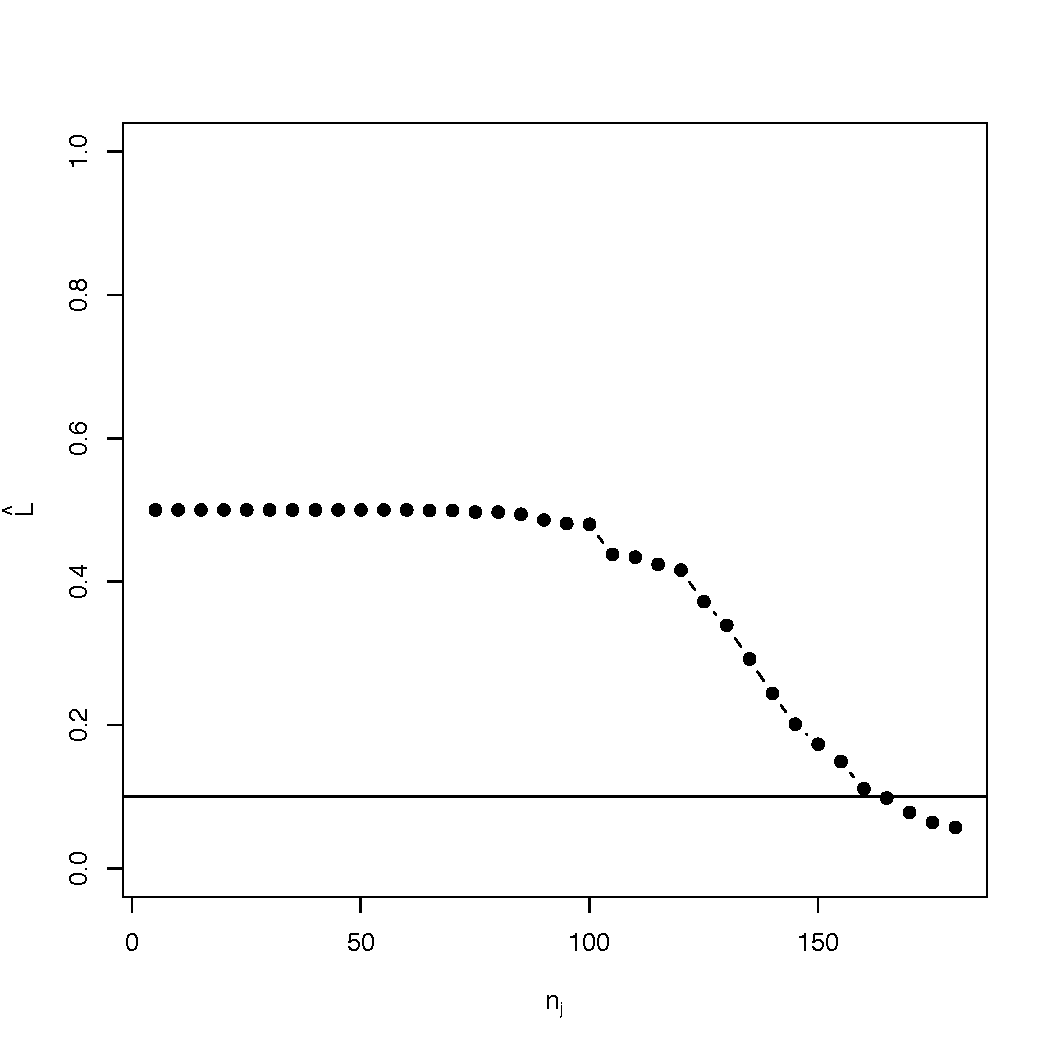
\includegraphics[width=.5\linewidth]{Lhatplot}
\caption{C.~elegans graph classification simulation results. $\hL^{1000}_{F}(g_n)$ is plotted as a function of class-conditional training sample size $n_j$, suggesting that for $\varepsilon=0.1$ we can determine that $\MeB$ holds with $99\%$ confidence with just a few hundred training samples generated from $F_{BM}$. Each dot depicts an estimate for $L_{F}(g_n)$; standard errors are $(L_{F}(g_n)(1-L_{F}(g_n))/1000)^{1/2}$. E.g., $n_j = 180$ ; $k_n = 53$ ; $\hL^{1000}_{F}(g_n) = 0.057$; standard error less than 0.01. We reject $H_0: L_{F}(g^*) \geq 0.10$ at $\alpha=0.01$. $L_{F}(g^*) \approx 0$ for this simulation.}
\label{fig1}
\end{figure}


% section results (end)

\section{Discussion} % (fold)
\label{sec:discussion}

% section discussion (end)
\paragraph{Acknowledgments}

This research was partially supported by the NSA Research Program in Applied Neuroscience


\appendix
% \input{appendix}
% \clearpage

\bibliography{/Users/joshyv/Research/misc/biblist}
\addcontentsline{toc}{section}{References}
%\bibliographystyle{apalike}
\bibliographystyle{ieeetr}
%\bibliographystyle{nature}

\end{document}
